\section{Equalizers}\label{sec:equalizer}

En equalizer er et form for filter der har til formål at 
udglatte et givent signal. I modsætning til filtre der normalt designes til et specifikt formål
 er equalizeren justerbar og kan tilpasses alt afhængig af det signal der påtrykkes og hvilket formål
 der ønskes.\\
Der er to hovedgrupper af equalizers: Grafisk Equalizers og Parametriske Equalizers.\\
Der er uenighed i definitionerne af de to typer, hvilket medfører forvirring omkring specifikationer af filter.
I denne rapport vælges følgende definitioner:
\begin{itemize}
\item Grafisk Equalizer: Her splittes equalizeren op i forskellige bånd der dækker sine respektive
frekvens områder. Som bruger har man forstærkning som parameter at ændre på. 
Båndbredde og center frekvens er fastlagt.
\item Parametrisk Equalizer: Her er båndende vilkårlige således at brugeren selv kan
tilføje og fjerne dem efter behov. I hvert enkelt bånd kan man justere båndbredde, center frekvens
og forstærkning ved center frekvensen. 
\end{itemize}  


\begin{figure}
	\centering
	\subbottom[]{%
  		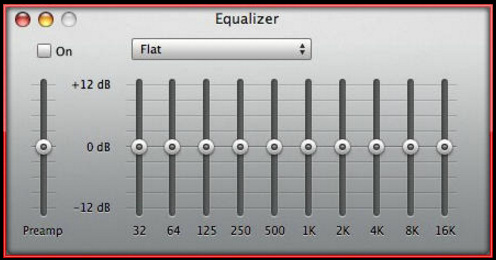
\includegraphics[width=.39\textwidth]{billeder/grafisk_eq_ill.png}
	  	\label{fig:graf_eq_ill}}
	\subbottom[]{%
		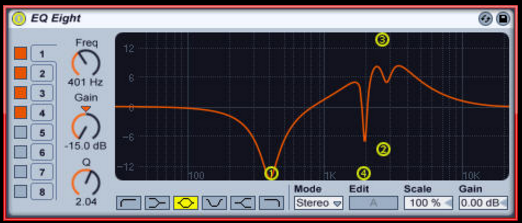
\includegraphics[width=.45\textwidth]{billeder/param_eq_ill.png}
		\label{fig:param_eq_ill}}
  	\caption{\ref{fig:graf_eq_ill} viser en grafisk equalizer, \ref{fig:param_eq_ill} viser en parametrisk equalizer.}
	\label{fig:eq_ill}
\end{figure}
\FloatBlock

Af de to typer er den parametriske klart den mest fleksible men
også mere beregningstung. På figur \ref{fig:eq_ill}
kan der tydeligt ses forskel f.eks. har filteret \ref{fig:param_eq_ill}
nogle frekvens specifikationer som den grafiske equalizer ikke kan realiserer.\\

Equalizers bruges i studio teknik, radio teknik, telefoni, forbruger-audioforstærkerer. 
